%%%%%%%%%%%%%%%%%%%%%%%%%%%%%%%%%%%%%%%%%%%%%%%%%%%%%%%%%%%%%%%%%%%%%%%%%%%%%%%%%%
\begin{frame}[fragile]\frametitle{}
\begin{center}
{\Large Mental Models}

{\small Farnam Street - Shane Parrish}


\end{center}
\end{frame}



%%%%%%%%%%%%%%%%%%%%%%%%%%%%%%%%%%%%%%%%%%%%%%%%%%%%%%%%%%%
\begin{frame}[fragile]\frametitle{}

\begin{center}
{\it 
``What the pupil must learn, if he learns anything at all, is that the world will do most of the work for you, provided you cooperate with it by identifying how it really works and aligning with those realities. If we do not let the world teach us, it teaches us a lesson.''


— Joseph Tussman
}

\end{center}
	  
\end{frame}

%%%%%%%%%%%%%%%%%%%%%%%%%%%%%%%%%%%%%%%%%%%%%%%%%%%%%%%%%%%%%%%%%%%%%%%%%%%%%%%%%%
\begin{frame}[fragile]\frametitle{}
\begin{center}
{\large A Framework for Making Smarter Decisions and Fewer Errors}

{\small Farnam Street - Shane Parrish}


\end{center}
\end{frame}



%%%%%%%%%%%%%%%%%%%%%%%%%%%%%%%%%%%%%%%%%%%%%%%%%%%%%%%%%%%
\begin{frame}[fragile]\frametitle{Why Mental Models?}

\begin{itemize}
\item No one Taught you How to Decide
\item There is no class called ``decision making''. 
\item It isn’t one skill but rather a series of tools and frameworks.
\item We use same tool for any problem that comes to us.
\item Need to develop tool box of various mental models
\end{itemize}

\end{frame}


%%%%%%%%%%%%%%%%%%%%%%%%%%%%%%%%%%%%%%%%%%%%%%%%%%%%%%%%%%%
\begin{frame}[fragile]\frametitle{Mistakes made by the famous}

\begin{itemize}
\item Napoleon deciding to invade Russia (and Hitler doing it again 130 years later)
\item NASA’s decision to ignore the O-ring issues on the Challenger
\item Juergen Schrempp, the CEO of Daimler-Benz, deciding to merge with Chrysler despite massive internal opposition and a general history of big M\&A deals working very poorly
\item  [YK] Italian Mayor starting campaign to start hugging Chinese tourists, to show 'SOLIDARITY' proved fatal wrt CORONA outbreak
\end{itemize}

\end{frame}


%%%%%%%%%%%%%%%%%%%%%%%%%%%%%%%%%%%%%%%%%%%%%%%%%%%%%%%%%%%
\begin{frame}[fragile]\frametitle{Sources of Stupidity}
\begin{itemize}
\item unintentional: when tired, overly focused on a goal, rushing, distracted, operating in a group, or under the influence of a group
\item have the wrong information
\item use the wrong model
\item fail to learn
\item trying to look better than doing good
\end{itemize}

[YK] murkha lakshan and padhat murkha by Ramdas

\end{frame}


%%%%%%%%%%%%%%%%%%%%%%%%%%%%%%%%%%%%%%%%%%%%%%%%%%%%%%%%%%%
\begin{frame}[fragile]\frametitle{Intelligent Preparation: The World Is Multidisciplinary}


If you're going to compete with people, you want to compete with people who are way less sophisticated than you.

\begin{itemize}
\item Inversion — Otherwise known as thinking something through in reverse or thinking ``backwards'', inversion is a problem-solving technique.
\item Second-Order Thinking - Ask yourself, ``And then what?”''
\item The Map Is Not the Territory —The map of reality is not reality itself. If any map were to represent its actual territory with perfect fidelity, it would be the size of the territory itself.
\end{itemize}

e.g. Sexy Internet businesses are rarely effective, no matter how good they are, because the others are nearly just as good. What you want is contrast — to be the big fish in a small pond.
\end{frame}

%%%%%%%%%%%%%%%%%%%%%%%%%%%%%%%%%%%%%%%%%%%%%%%%%%%%%%%%%%%
\begin{frame}[fragile]\frametitle{Charile Munger}

has about 100 models, some examples:

\begin{itemize}
\item Redundancy/backup system model from engineering.
\item Compound interest from mathematics
\item The breakpoint/autocatalysis from chemistry/physics.
\item Modern Darwinian synthesis from biology.
\item Cognitive misjudgment from psychology.
\end{itemize}

Combination of models AND application of them together = critical mass, they reinforce and amplify each other. (“Lollapalooza effect”).

\end{frame}


%%%%%%%%%%%%%%%%%%%%%%%%%%%%%%%%%%%%%%%%%%%%%%%%%%%%%%%%%%%
\begin{frame}[fragile]\frametitle{Fair Division}
\begin{columns}
    \begin{column}[T]{0.6\linewidth}
      \begin{itemize}
		\item Problem: While distributing a cake between two brothers, the younger feels that the elder one is cutting into unequal chunks and taking the bigger piece.
		\item Core Issue: Division and Allocation is done by same person.
		\item Solution: Separate both. Meaning, one of them cuts the cake and the other picks. So, almost no chance that the one who divides will make unequal pieces!!
	  \end{itemize}

    \end{column}
    \begin{column}[T]{0.4\linewidth}
		\begin{center}
		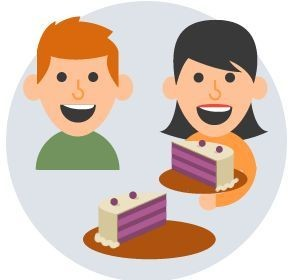
\includegraphics[width=0.8\linewidth,keepaspectratio]{images/game_theory_fair_division}
		
		{\small ``I-Cut-You-Choose'' Cake-Cutting Protocol Inspires Solution to Gerrymandering - 
Byron Spice (SCS) and Jocelyn Duffy (MCS)}
		\end{center}	
    \end{column}
  \end{columns}
\end{frame}

%%%%%%%%%%%%%%%%%%%%%%%%%%%%%%%%%%%%%%%%%%%%%%%%%%%%%%%%%%%%%%%%%%%%%%%%%%%
\begin{frame}[fragile]\frametitle{References}
\begin{itemize}
\item Farnam Street, Mendtal Models https://fs.blog/mental-models/

\item Farnam Street, How To Deciside: https://fs.blog/smart-decisions/\#how\_to\_decide
\end{itemize}
\end{frame}